\documentclass[handout,x11names]{beamer}
\usepackage{etex,beamerfoils}
\usepackage{array,pifont,amsmath,latexsym,epsfig,amsfonts,yfonts}
\usepackage{amstext,amsopn,amsxtra,amsgen,amsbsy,amscd,amssymb,dcolumn,graphicx,setspace,pgfplots,booktabs,natbib}
\usepackage[normalem]{ulem}
\usepackage[all]{xy}
\beamertemplatetheoremsnumbered
\setbeamertemplate{caption}[numbered]
\usetheme{Copenhagen}
\definecolor{NewBlue}{RGB}{4, 114, 155}
\definecolor{magenta}{cmyk}{0,1,0,0}
\usecolortheme[named=NewBlue]{structure}
%\usecolortheme[named=SkyBlue4]{structure}


\newcommand{\D}{\displaystyle}
\newcommand{\E}{\begin{eqnarray*}}
\newcommand{\F}{\end{eqnarray*}}
\newcommand{\EE}{\begin{eqnarray}}
\newcommand{\FF}{\end{eqnarray}}
\newcommand{\IZ}{\begin{itemize}}
\newcommand{\ZI}{\end{itemize}}
\newcommand{\EN}{\begin{enumerate}}
\newcommand{\NE}{\end{enumerate}}
\newcommand{\itemc}{\item[$\circ$]}
\newcommand{\IZdash}{\begin{itemize} \renewcommand{\labelitemi}{-}}
\newcommand{\tn}{\textnormal}

% New commands to assist Beamer
\newcommand{\itemi}{\item<1->}
\newcommand{\itemii}{\item<2->}
\newcommand{\itemiii}{\item<3->}
\newcommand{\itemiv}{\item<4->}
\newcommand{\itemv}{\item<5->}
\newcommand{\itemvi}{\item<6->}
\newcommand{\itemvii}{\item<7->}
\newcommand{\itemviii}{\item<8->}
\newcommand{\itemix}{\item<9->}
\newcommand{\itemx}{\item<10->}

\newcommand{\itemci}{\item[$\circ$]<1->}
\newcommand{\itemcii}{\item[$\circ$]<2->}
\newcommand{\itemciii}{\item[$\circ$]<3->}
\newcommand{\itemciv}{\item[$\circ$]<4->}
\newcommand{\itemcv}{\item[$\circ$]<5->}
\newcommand{\itemcvi}{\item[$\circ$]<6->}
\newcommand{\itemcvii}{\item[$\circ$]<7->}
\newcommand{\itemcviii}{\item[$\circ$]<8->}
\newcommand{\itemcix}{\item[$\circ$]<9->}
\newcommand{\itemcx}{\item[$\circ$]<10->}


\newcommand{\fr}{\frame}
\newcommand{\ft}{\frametitle}
\newcommand{\ons}{\onslide}
\newcommand{\tc}{\textcolor}

\pgfplotsset{height =7cm,compat=1.7,width=7cm,
    standard/.style={
    	unit vector ratio*=1 1 1,
        axis x line=middle,
        axis y line=middle,
        enlarge x limits=0.15,
        enlarge y limits=0.15,
        every axis x label/.style={at={(current axis.right of origin)},anchor=north west},
        every axis y label/.style={at={(current axis.above origin)},anchor=north east}
    }
}
\newcommand{\drawge}{-- (rel axis cs:1,0) -- (rel axis cs:1,1) -- (rel axis cs:0,1) \closedcycle}
\newcommand{\drawle}{-- (rel axis cs:1,1) -- (rel axis cs:1,0) -- (rel axis cs:0,0) \closedcycle}

\usetikzlibrary{patterns}
\usetikzlibrary{arrows}
\usetikzlibrary{shapes}

\renewcommand{\bibsection}{}

% Watermark example: https://texblog.org/2012/02/17/watermarks-draft-review-approved-confidential/
\usepackage{draftwatermark}
\SetWatermarkText{This content is protected and may not be shared uploaded or distributed.}
\SetWatermarkScale{0.25}
\SetWatermarkAngle{0}
\SetWatermarkColor[gray]{1.0}
\setbeamercolor{background canvas}{bg=}%transparent canvas

\title[Pandas and Statsmodels\hspace{2em}\insertframenumber/
\inserttotalframenumber]{Pandas and Statsmodels}
\author[Brian C. Jenkins - Computational Macroeconomics ]{Brian C.~Jenkins \\ ~ \\Econ 126: Computational Macroeconomics\\ ~ \\University of California, Irvine}

\begin{document}

\frame{\maketitle}


\fr{
\ft{Background}
\IZ
\item Recall human capital-augmented Cobb-Douglas production function:
\begin{align}
Y & = A K^{\alpha}\left(hL\right)^{1-\alpha}, \label{eqn:production}
\end{align}
where:
	\IZ
	\itemii $Y$: production of final goods and services
	\itemiii $K$: stock of physical capital
	\itemiv $L$: labor force
	\itemv $h$: human capital \emph{per worker}
	\itemvi $A$ \emph{total factor productivity} or TFP
	\ZI
\ZI
}


\fr{
\ft{Background}
\IZ
\item In the production function, every variable \emph{except} $A$ is \emph{measured}:

	\IZ
	\itemii $Y$ measured by (real) GDP
	\itemiii $K$: inferred from investment and depreciation data
	\itemiv $L$: measured as number of workers or number of worker hours
	\itemv $h$: typically measured as average years of education
	\ZI
	
\

\itemvi Of course macroeconomic measurement is subject to \emph{measurement error}.
\ZI
}

\fr{
\ft{Background}
\IZ
\item The production function \emph{implies} a value for $A$:

\begin{align}
A & = \frac{Y}{K^{\alpha}(hL)^{1-\alpha}}
\end{align}

\

\itemii $A$ captures all other determinants of production that are not reflected in $K$, $L$, or $h$. For example:
	\IZ
	\itemiii Quality of economic and political institutions
	\itemiv Degree of technology adoption
	\itemv Public health
	\ZI
\ZI
}






\fr{
\begin{figure}[h] \caption{\label{fig2} \textbf{TFP and GDP per capita across countries.} All values relative to the US. Source: \cite{JonesRomer2010} }
\hspace*{-.5cm}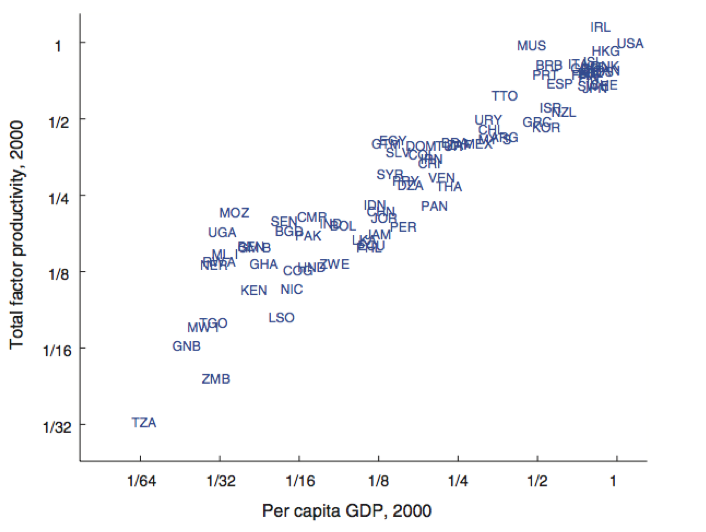
\includegraphics[height = 5cm]{external_fig_08_New_Kaldor_Facts_Jones_Romer_Fig4.png}
\end{figure}
}


\fr{
\ft{Jones and Romer (2010)}
\IZ
\item \emph{Even after accounting for their lower levels of human capital per worker and physical capital per worker}, workers in lower-income countries are less productive

\

\itemii Workers in lower-income countries use what human and physical capital the \emph{do} have less efficiently than workers in higher-income countries. 

\

\itemiii Since TFP isn't directly observable, we still don't know exactly why.
\ZI
}


\fr{
\ft{References}
\bibliographystyle{aer}
\bibliography{comp_econ_references.bib}
}




\end{document}